\documentclass[a4paper]{article}
\usepackage{longtable,float,hyperref,color,amsmath,amsxtra,amssymb,latexsym,amscd,amsthm,amsfonts,graphicx}
\numberwithin{equation}{section}
\allowdisplaybreaks
\usepackage{fancyhdr}
\pagestyle{fancy}
\fancyhf{}
\fancyhead[RE,LO]{\footnotesize \textsc \leftmark}
\cfoot{\thepage}
\renewcommand{\headrulewidth}{0.5pt}
\setcounter{tocdepth}{3}
\setcounter{secnumdepth}{3}
\usepackage{imakeidx}
\makeindex[columns=2, title=Alphabetical Index, 
           options= -s index.ist]
\title{\huge Differential Geometry 004\\
An Introduction to Conformal Mapping}
\author{\textsc{Nguyen Quan Ba Hong}\footnote{Student ID. 1411103}\\
\textsc{Doan Tran Nguyen Tung}\footnote{Student ID. 1411352}\\
\textsc{Nguyen An Thinh}\footnote{Student ID. 1411289}\\
{\small Students at Faculty of Math and Computer Science}\\ 
{\small Ho Chi Minh University of Science, Vietnam} \\
{\small \texttt{email. nguyenquanbahong@gmail.com}}\\
{\small \texttt{email. dtrngtung@live.com}}\\
{\small \texttt{email. anthinh297@gmail.com}}\\
{\small \texttt{blog. \url{www.nguyenquanbahong.com}} 
\footnote{Copyright \copyright\ 2016-2018 by Nguyen Quan Ba Hong, Student at Ho Chi Minh University of Science, Vietnam. This document may be copied freely for the purposes of education and non-commercial research. Visit my site \texttt{\url{www.nguyenquanbahong.com}} to get more.}}}
\begin{document}
\maketitle
\begin{abstract}
In this context, we introduce the notion of conformal mapping and some basic properties  of this notion in differential geometry.
\end{abstract}
\newpage
\tableofcontents
\newpage
\section{Introduction}
In the definition of the angle between two tangent vectors $X,Y$,
\begin{align}
\cos \varphi  = \frac{{\left\langle {X,Y} \right\rangle }}{{\left\| X \right\| \cdot \left\| Y \right\|}},
\end{align}
only the value of the inner product $\left\langle {X,Y} \right\rangle $ in relation to the length of both vectors occurs. Therefore the angle is preserved if both are multiplied by the same factor. This is precisely what characterizes an ``angle preserving mapping''.\\
\\
\textbf{Definition 1.1 (Conformal Parametrization).} (\cite{1}, Definition 3.29, p.101) A parametrization $f:U\to \mathbb{R}^3$ of a surface element is called \textit{conformal} or \textit{angle preserving}, if the first fundamental form, written in these parameters, is a scalar multiple of the unit matrix, i.e., if the equation
\begin{align}
\left( {{g_{ij}}} \right) = \lambda \left( {{u_1},{u_2}} \right)\left( {\begin{array}{*{20}{c}}
1&0\\
0&1
\end{array}} \right)
\end{align} 
holds for some function $\lambda :U\to \mathbb{R}$. More generally, two surface elements which are parametrized by the same set $f, \widetilde{f}: U\to \mathbb{R}^3$ are said to be \textit{conformally equivalent}, if the first fundamental form $\left(g_{ij}\right)$ of one of them is a scalar multiple of the other $\left(\widetilde{g_{ij}}\right)$:
\begin{align}
\label{1.3}
\left( {\widetilde {{g_{ij}}}} \right) = \lambda \left( {{u_1},{u_2}} \right)\left( {{g_{ij}}} \right),\hspace{0.2cm}\left( {{u_1},{u_2}} \right) \in U,
\end{align}
with some positive function $\lambda :U\to \mathbb{R}$. A similar statement holds after a change of parameters: $f:U\to \mathbb{R}^3, \widetilde{f}:\widetilde{U}\to \mathbb{R}^3$ are said to be \textit{conformally equivalent} with the \textit{conformal factor} $\lambda$, if there is a change of parametrizations $\Phi :U \to \widetilde U$ such that 
\begin{align}
\left\langle {\frac{{\partial \left( {\widetilde f \circ \Phi } \right)}}{{\partial {u_i}}},\frac{{\partial \left( {\widetilde f \circ \Phi } \right)}}{{\partial {u_j}}}} \right\rangle  = \lambda \left( {{u_1},{u_2}} \right) \cdot \left\langle {\frac{{\partial f}}{{\partial {u_i}}},\frac{{\partial f}}{{\partial {u_j}}}} \right\rangle \mbox{ for all } i,j.
\end{align}
A conformal parametrization is also called \textit{isothermal}, and the parameters are also referred to as \textit{isothermal coordinates}. The notion of angles is then identical with that in the Euclidean space $\left(u_1,u_2\right)$-plane.\\

When dealing with problems associated with analytic functions of complex variables, it is important to introduce the conformal equivalence. We also give below an alternative definition of the notion of conformal mapping for completeness.\\
\\
\textbf{Definition 1.2.} (Definition 3, \cite{2}, p.226) Let $S,\overline{S}$ be regular surfaces, a diffeomorphism $\varphi: S\to \overline{S}$ is called a \textit{conformal map} if for all $p\in S$ and all $v_1,v_2\in T_p\left(S\right)$ we have
\begin{align}
\label{1.5}
\left\langle {d{\varphi _p}\left( {{v_1}} \right),d{\varphi _p}\left( {{v_2}} \right)} \right\rangle  = {\lambda ^2}\left( p \right){\left\langle {{v_1},{v_2}} \right\rangle _p},
\end{align}
when $\lambda ^2$ is a nowhere-zero differentiable function on $S$; the surfaces $S$ and $\overline{S}$ are then said to be \textit{conformal}. A map $\varphi:V\to \overline{S}$  of a neighborhood $V$ of $p\in S$ into $\overline{S}$ is a \textit{local conformal map} at $p$ if there exists a neighborhood $\overline{V}$ of $\varphi \left(p\right)$ such that $\varphi :V\to \overline{V}$ is a conformal map. If for each $p\in S$, there exists a local conformal map at $p$, the surface $S$ is said to be \textit{locally conformal} to $\overline{S}$.\\

The geometric meaning of the above definition is that the angles (but not necessarily the lengths) are preserved by conformal maps. In fact, let $\alpha :I\to S$ and $\beta :I\to S$ be two curves in $S$ which intersect at, say, $t=0$. Their angle $\theta$ at $t=0$ is given by
\begin{align}
\cos \theta  = \frac{{\left\langle {\alpha ',\beta '} \right\rangle }}{{\left\| {\alpha '} \right\|\left\| {\beta '} \right\|}},\hspace{0.2cm}0 < \theta  < \pi .
\end{align}
A conformal map $\varphi :S\to \overline{S}$ maps these curves into curves $\varphi  \circ \alpha :I \to \overline S $, $\varphi  \circ \beta :I \to \overline S $, which intersect for $t=0$, making an angle $\overline{\theta}$ given by
\begin{align}
\cos \overline \theta   = \frac{{\left\langle {d\varphi \left( {\alpha '} \right),d\varphi \left( {\beta '} \right)} \right\rangle }}{{\left\| {d\varphi \left( {\alpha '} \right)} \right\|\left\| {d\varphi \left( {\beta '} \right)} \right\|}} = \frac{{{\lambda ^2}\left\langle {\alpha ',\beta '} \right\rangle }}{{{\lambda ^2}\left\| {\alpha '} \right\|\left\| {\beta '} \right\|}} = \cos \theta ,
\end{align}
as we claimed. It is not hard to prove this properties characterizes the locally conformal maps see Exercise 14, \cite{2}, p.229, or Problem 3.4 in this context.

\section{Some Basic Properties of Conformal Mappings}
In this section, we collect some basic results in \cite{1} and \cite{2}.\\
\\
\textbf{Theorem 2.1.} (\cite{1}, Consequence 3.30, p.102) 
\begin{enumerate}
\item \textit{The Gauss map $\nu$ is conformal for a minimal surface with $K\ne 0$, i.e., $\nu$ and $f$ are conformally equivalent, with conformal factor $-K$.}
\item \textit{The following relation holds for a conformal parametrization $f:U\to \mathbb{R}^3$ with $\left( {{g_{ij}}} \right) = \lambda \left( {\begin{array}{*{20}{c}}
1&0\\
0&1
\end{array}} \right)$:}
\begin{align}
\frac{{{\partial ^2}f}}{{\partial u_1^2}} + \frac{{{\partial ^2}f}}{{\partial u_2^2}} = 2H\lambda  \cdot \nu .
\end{align}
\textit{In particular, a conformal parametrization $f$ defines a minimal surface if and only if the three component functions $f_1,f_2,f_3$ of $f$ are harmonic, which means that the relation}
\begin{align}
\Delta {f_i} = \frac{{{\partial ^2}{f_i}}}{{\partial u_1^2}} + \frac{{{\partial ^2}{f_i}}}{{\partial u_2^2}} = 0
\end{align}
\textit{holds. The vector $\mathbf{H}=H\cdot \nu$ is also called the \textbf{mean curvature vector}.}
\end{enumerate}
\textsc{Proof.} 
\begin{enumerate}
\item The first statement follows immediately from the equation 
\begin{align}
III-2H\cdot II+K\cdot I=0,
\end{align}
which implies that $III=-K\cdot I$. But $III$ is the first fundamental form of the map $\nu$.
\item For the second statement we start with the observation
\begin{align}
\left\langle {\frac{{\partial f}}{{\partial {u_1}}},\frac{{\partial f}}{{\partial {u_1}}}} \right\rangle & = \left\langle {\frac{{\partial f}}{{\partial {u_2}}},\frac{{\partial f}}{{\partial {u_2}}}} \right\rangle  = \lambda ,\\
\left\langle {\frac{{\partial f}}{{\partial {u_1}}},\frac{{\partial f}}{{\partial {u_2}}}} \right\rangle  &= 0.
\end{align}
By further differentiating it follows from this that
\begin{align}
\left\langle {\frac{{{\partial ^2}f}}{{\partial u_1^2}},\frac{{\partial f}}{{\partial {u_1}}}} \right\rangle  = \left\langle {\frac{{{\partial ^2}f}}{{\partial {u_1}\partial {u_2}}},\frac{{\partial f}}{{\partial {u_2}}}} \right\rangle  =  - \left\langle {\frac{{\partial f}}{{\partial {u_1}}},\frac{{{\partial ^2}f}}{{\partial u_2^2}}} \right\rangle .
\end{align}
We conclude $\left\langle {\frac{{{\partial ^2}f}}{{\partial u_1^2}} + \frac{{{\partial ^2}f}}{{\partial u_2^2}},\frac{{\partial f}}{{\partial {u_1}}}} \right\rangle  = 0$, and similarly $\left\langle {\frac{{{\partial ^2}f}}{{\partial u_1^2}} + \frac{{{\partial ^2}f}}{{\partial u_2^2}},\frac{{\partial f}}{{\partial {u_2}}}} \right\rangle  = 0$. Hence the vector ${\frac{{{\partial ^2}f}}{{\partial u_1^2}} + \frac{{{\partial ^2}f}}{{\partial u_2^2}}}$ is perpendicular to the tangent plane, thus linearly dependent on the unit normal $\nu$. But since 
\begin{align}
2H = \frac{{{g_{22}}{h_{11}} + {g_{11}}{h_{22}}}}{{{\lambda ^2}}} = \frac{{{h_{11}} + {h_{22}}}}{\lambda },
\end{align}
we have finally
\begin{align}
\left\langle {\frac{{{\partial ^2}f}}{{\partial u_1^2}} + \frac{{{\partial ^2}f}}{{\partial u_2^2}},\nu } \right\rangle  = {h_{11}} + {h_{22}} = 2H\lambda .
\end{align}
\end{enumerate}
This completes our proof. \hfill $\square$\\
\\
\textbf{Theorem 2.2 (Complexification).} (\cite{1}, Corollary 3.31, p.103) \textit{For a surface element $f:U\to \mathbb{R}^3$ with components $f=\left(f_1,f_2,f_3\right)$ we define the map $\varphi:U\to \mathbb{C}^3$ by the relation}
\begin{align}
\varphi \left( {u + iv} \right) = \frac{{\partial f}}{{\partial u}}\left( {u,v} \right) - i\frac{{\partial f}}{{\partial v}}\left( {u,v} \right),
\end{align}
\textit{which is, in components,}
\begin{align}
{\varphi _1}\left( {u + iv} \right) &= \frac{{\partial {f_1}}}{{\partial u}}\left( {u,v} \right) - i\frac{{\partial {f_1}}}{{\partial v}}\left( {u,v} \right),\\
{\varphi _2}\left( {u + iv} \right) &= \frac{{\partial {f_2}}}{{\partial u}}\left( {u,v} \right) - i\frac{{\partial {f_2}}}{{\partial v}}\left( {u,v} \right),\\
{\varphi _3}\left( {u + iv} \right) &= \frac{{\partial {f_3}}}{{\partial u}}\left( {u,v} \right) - i\frac{{\partial {f_3}}}{{\partial v}}\left( {u,v} \right).
\end{align}
\textit{Then, we have}
\begin{enumerate}
\item \textit{$f$ is conformal if and only if $\varphi _1^2 + \varphi _2^2 + \varphi _3^2 = 0$.}
\item \textit{If $f$ is a conformal parametrization, $f$ is a minimal surface if and only if the functions $\varphi _1,\varphi _2,\varphi _3$ are complex analytic (holomorphic).}
\item \textit{If conversely $\varphi _1,\varphi _2,\varphi _3$ are complex analytic with $\varphi _1^2 + \varphi _2^2 + \varphi _3^2 = 0$, then the function $f$ defined by the above equation is regular (hence an immersion) if and only if}
\begin{align}
{\varphi _1}\overline {{\varphi _1}}  + {\varphi _2}\overline {{\varphi _2}}  + {\varphi _3}\overline {{\varphi _3}}  \ne 0.
\end{align}
\end{enumerate}
\textsc{Proof.} 
\begin{enumerate}
\item By definition we have
\begin{align}
\varphi _1^2 + \varphi _2^2 + \varphi _3^2 &= \left\langle {\frac{{\partial f}}{{\partial u}},\frac{{\partial f}}{{\partial u}}} \right\rangle  + {i^2}\left\langle {\frac{{\partial f}}{{\partial v}},\frac{{\partial f}}{{\partial v}}} \right\rangle  - 2i\left\langle {\frac{{\partial f}}{{\partial u}},\frac{{\partial f}}{{\partial v}}} \right\rangle \\
 &= {g_{11}} - {g_{22}} - 2i{g_{12}}.
\end{align}
Thus the left hand side vanishes if and only if $g_{11}=g_{22}$ and $g_{12}=0$ hold.
\item We calculate the second derivatives
\begin{align}
\frac{{{\partial ^2}{f_k}}}{{\partial {u^2}}} &= \frac{\partial }{{\partial u}}\left( {{\mathop{\rm Re}\nolimits} {\varphi _k}} \right),\\
\frac{{{\partial ^2}{f_k}}}{{\partial {v^2}}} &=  - \frac{\partial }{{\partial v}}\left( {{\mathop{\rm Im}\nolimits} {\varphi _k}} \right),\\
\frac{{{\partial ^2}{f_k}}}{{\partial u\partial v}} &= \frac{\partial }{{\partial v}}\left( {{\mathop{\rm Re}\nolimits} {\varphi _k}} \right) =  - \frac{\partial }{{\partial u}}\left( {{\mathop{\rm Im}\nolimits} {\varphi _k}} \right).
\end{align}
The validity of the equation $\frac{{{\partial ^2}f}}{{\partial {u^2}}} + \frac{{{\partial ^2}f}}{{\partial {v^2}}} = 0$ is then equivalent to the validity of the Cauchy-Riemann equations (abbr., CR-equations) for $\varphi _1,\varphi _2,\varphi _3$. By Theorem 2.1, this is precisely the case when $f$ is a minimal surface.
\item We have 
\begin{align}
{\varphi _1}\overline {{\varphi _1}}  + {\varphi _2}\overline {{\varphi _2}}  + {\varphi _3}\overline {{\varphi _3}}  = \left\langle {\frac{{\partial f}}{{\partial u}},\frac{{\partial f}}{{\partial u}}} \right\rangle  + \left\langle {\frac{{\partial f}}{{\partial v}},\frac{{\partial f}}{{\partial v}}} \right\rangle  \ge 0,
\end{align}
with equality if and only if $\frac{{\partial f}}{{\partial u}} = \frac{{\partial f}}{{\partial v}} = 0$. By the proof of $\left(1\right)$, either both vectors vanish or both are non-vanishing and linearly independent. This implies $\left(3\right)$. \hfill $\square$
\end{enumerate} 
The zeros of the complex map $\varphi$ corresponds by $\left(3\right)$ to the points at which $f$ is not regular (so-called singularities of $f$). The reason for these considerations is that in the theory of functions of a complex variable it does not make sense to exclude zeros, while in differential geometry one usually assumes regular surface elements.\\
\\
\textbf{Lemma 2.3 (Isothermal coordinates)} (\cite{1}, Lemma 3.33, p.105) \textit{In lines of curvature parameters $\left(u_1,u_2\right)$ for a minimal surface with $K\ne 0$ (this means $g_{12}=h_{12}=0$), one can construct by a simple integration a conformal parametrization, that is, isothermal coordinates.}\\
\\
\textsc{Proof.} In lines of curvature parameters we have
\begin{align}
\frac{{\partial \nu }}{{\partial {u_i}}} =  - {\kappa _i}\frac{{\partial f}}{{\partial {u_i}}},
\end{align}
hence
\begin{align}
\frac{{{\partial ^2}\nu }}{{\partial {u_1}\partial {u_2}}} =  - \frac{\partial }{{\partial {u_1}}}\left( {{\kappa _2} \cdot \frac{{\partial f}}{{\partial {u_2}}}} \right) =  - \frac{\partial }{{\partial {u_2}}}\left( {{\kappa _1} \cdot \frac{{\partial f}}{{\partial {u_1}}}} \right).
\end{align}
If we now set $\kappa :=\kappa _1 =-\kappa _2>0$, it follows that
\begin{align}
\frac{{\partial \kappa }}{{\partial {u_2}}}\frac{{\partial f}}{{\partial {u_1}}} + 2\kappa \frac{{{\partial ^2}f}}{{\partial {u_1}\partial {u_2}}} + \frac{{\partial \kappa }}{{\partial {u_1}}}\frac{{\partial f}}{{\partial {u_2}}} = 0,
\end{align}
and hence
\begin{align}
\left\langle {\frac{{\partial \kappa }}{{\partial {u_2}}}\frac{{\partial f}}{{\partial {u_1}}} + 2\kappa \frac{{{\partial ^2}f}}{{\partial {u_1}\partial {u_2}}} + \frac{{\partial \kappa }}{{\partial {u_1}}}\frac{{\partial f}}{{\partial {u_2}}},\frac{{\partial f}}{{\partial {u_1}}}} \right\rangle  = 0;
\end{align}
consequently
\begin{align}
\frac{{\partial \kappa }}{{\partial {u_2}}}{g_{11}} + \kappa \frac{{\partial {g_{11}}}}{{\partial {u_2}}} + \frac{{\partial \kappa }}{{\partial {u_1}}} \cdot 0 = \frac{\partial }{{\partial {u_2}}}\left( {\kappa  \cdot {g_{11}}} \right) = 0.
\end{align}
It follows that $\kappa \cdot g_{11}$ is constant in the $u_2$-direction, hence it is a function of $u_1$ only. Similarly, $\kappa \cdot g_{22}$ is constant in the $u_1$-direction, hence a function of $u_2$ only. We now set $\kappa  \cdot {g_{11}} = {\Phi _1}\left( {{u_1}} \right) > 0$ and $\kappa  \cdot {g_{22}} = {\Phi _2}\left( {{u_2}} \right) > 0$ as well as ${v_i}: = \int {\sqrt {{\Phi _i}\left( {{u_i}} \right)} d{u_i}} $, $i=1,2$. Then the Jacobi matrix of the transformation $\left(u_1,u_2\right)\mapsto \left(v_1,v_2\right)$, which is
\begin{align}
\left( {\frac{{\partial {v_i}}}{{\partial {u_j}}}} \right) = \left( {\begin{array}{*{20}{c}}
{\sqrt {{\Phi _1}} }&0\\
0&{\sqrt {{\Phi _2}} }
\end{array}} \right),
\end{align}
is of maximal rank. The line element $ds^2$ transforms under this above transformation as follows:
\begin{align}
d{s^2} &= {g_{11}}du_1^2 + {g_{22}}du_2^2\\
& = \frac{{{\Phi _1}}}{\kappa }du_1^2 + \frac{{{\Phi _2}}}{\kappa }du_2^2\\
& = \frac{{{\Phi _1}}}{\kappa }{\left( {\frac{1}{{\sqrt {{\Phi _1}} }}d{v_1}} \right)^2} + \frac{{{\Phi _2}}}{\kappa }{\left( {\frac{1}{{\sqrt {{\Phi _2}} }}d{v_2}} \right)^2}\\
& = \frac{1}{\kappa }\left( {dv_1^2 + dv_2^2} \right).
\end{align}
Thus $v_1,v_2$ are isothermal coordinates, i.e., $I\left( {{v_1},{v_2}} \right) = \frac{1}{\kappa }\left( {\begin{array}{*{20}{c}}
1&0\\
0&1
\end{array}} \right)$. This holds whenever $f$ is a minimal surface without level points, i.e., in case $H\equiv 0$ and $K\ne 0$. It is easy to see that near a level point the factor $\frac{1}{\kappa}$ can become arbitrarily large and that this process will not work near such a point. \hfill $\square$\\

Every minimal surface locally allows a conformal parametrization, provided no level points occur. In this conformal parametrization the surface is analytic, occurring as the real part of a complex-analytic function. For a given $\varphi$ with the constraints $\left| \varphi  \right| \ne 0$ and $\varphi _1^2 + \varphi _2^2 + \varphi _3^2 = 0$, one even gets according to Corollary 3.32, \cite{1}, p.105 a completely explicit minimal surface. Furthermore, we can freely prescribe the function without the use of a constraint by using the so-called \textit{Weierstrass representation} which allows a more or less free choice of two functions.\\
\\
\textbf{Theorem 2.4 (Weierstrass representation).} (\cite{1}, Corollary 3.36, p.108) \textit{Every conformal parametrized minimal surface $f$ that is not a plane can locally be represented as follows:}
\begin{align}
{f_1}\left( z \right) &= {\mathop{\rm Re}\nolimits} \int_{{z_0}}^z {\frac{1}{2}F\left( \zeta  \right)\left( {1 - {G^2}\left( \zeta  \right)} \right)d\zeta } ;\\
{f_2}\left( z \right) &= {\mathop{\rm Re}\nolimits} \int_{{z_0}}^z {iF\left( \zeta  \right)\left( {1 + {G^2}\left( \zeta  \right)} \right)d\zeta } ;\\
{f_3}\left( z \right) &= {\mathop{\rm Re}\nolimits} \int_{{z_0}}^z {\frac{1}{2}F\left( \zeta  \right)G\left( \zeta  \right)d\zeta } ,
\end{align}
\textit{where $F$ is holomorphic and $G$ is meromorphic such that $FG^2$ is holomorphic. The domain of definition of the parametrization must be chosen in such a way that the occurring integrals are independent of the path of integration (for example, a small disc or a simply connected domain).}

\textit{Conversely, every pair $\left(F\left(\zeta
\right),G\left(\zeta \right)\right)$ with holomorphic $FG^2$ defines a conformal parametrized minimal surface element $f$. This $f$ is regular if $F$ has zeros only at the poles of $G$ and there it holds that $FG^2\ne 0$.}\\
\\
\textbf{Proposition 2.5.} \textit{Let $\mathbf{x}:U\to S$ and $\overline{\mathbf{x}}:U\to \overline{S}$ be parametrizations such that $E = \lambda {\overline E ^2},F = \lambda {\overline F ^2},G = \lambda {\overline G ^2}$ in $U$, where $\lambda^2$ is a nowhere-zero differentiable function in $U$. Then the map $\varphi  = \overline{\mathbf{x}}  \circ {\mathbf{x}^{ - 1}}:\mathbf{x}\left( U \right) \to \overline S $ is a local conformal map.}\\
\\
\textsc{Proof.} Let $p\in \mathbf{x}\left(U\right)$ and $w\in T_p\left(S\right)$. Then $w$ is tangent to a curve $\mathbf{x}\left(\alpha\left(t\right)\right)$ at $t=0$, where $\alpha\left(t\right) =\left(u\left(t\right),v\left(t\right)\right)$ is a curve in $U$; thus $w$ may be written ($t=0$)
\begin{align}
w = {\mathbf{x}_u}u' + {\mathbf{x}_v}v'.
\end{align}
By definition, the vector $\varphi _p\left(w\right)$ is the tangent vector to the curve $\overline{ \mathbf{x}}  \circ {\mathbf{x}^{ - 1}} \circ \overline{\mathbf{x}} \left( {\alpha \left( t \right)} \right)$, i.e., to the curve $\overline{\mathbf{x}}\left(\alpha \left(t\right)\right)$ at $t=0$, Figure 1.
\begin{figure}[H]
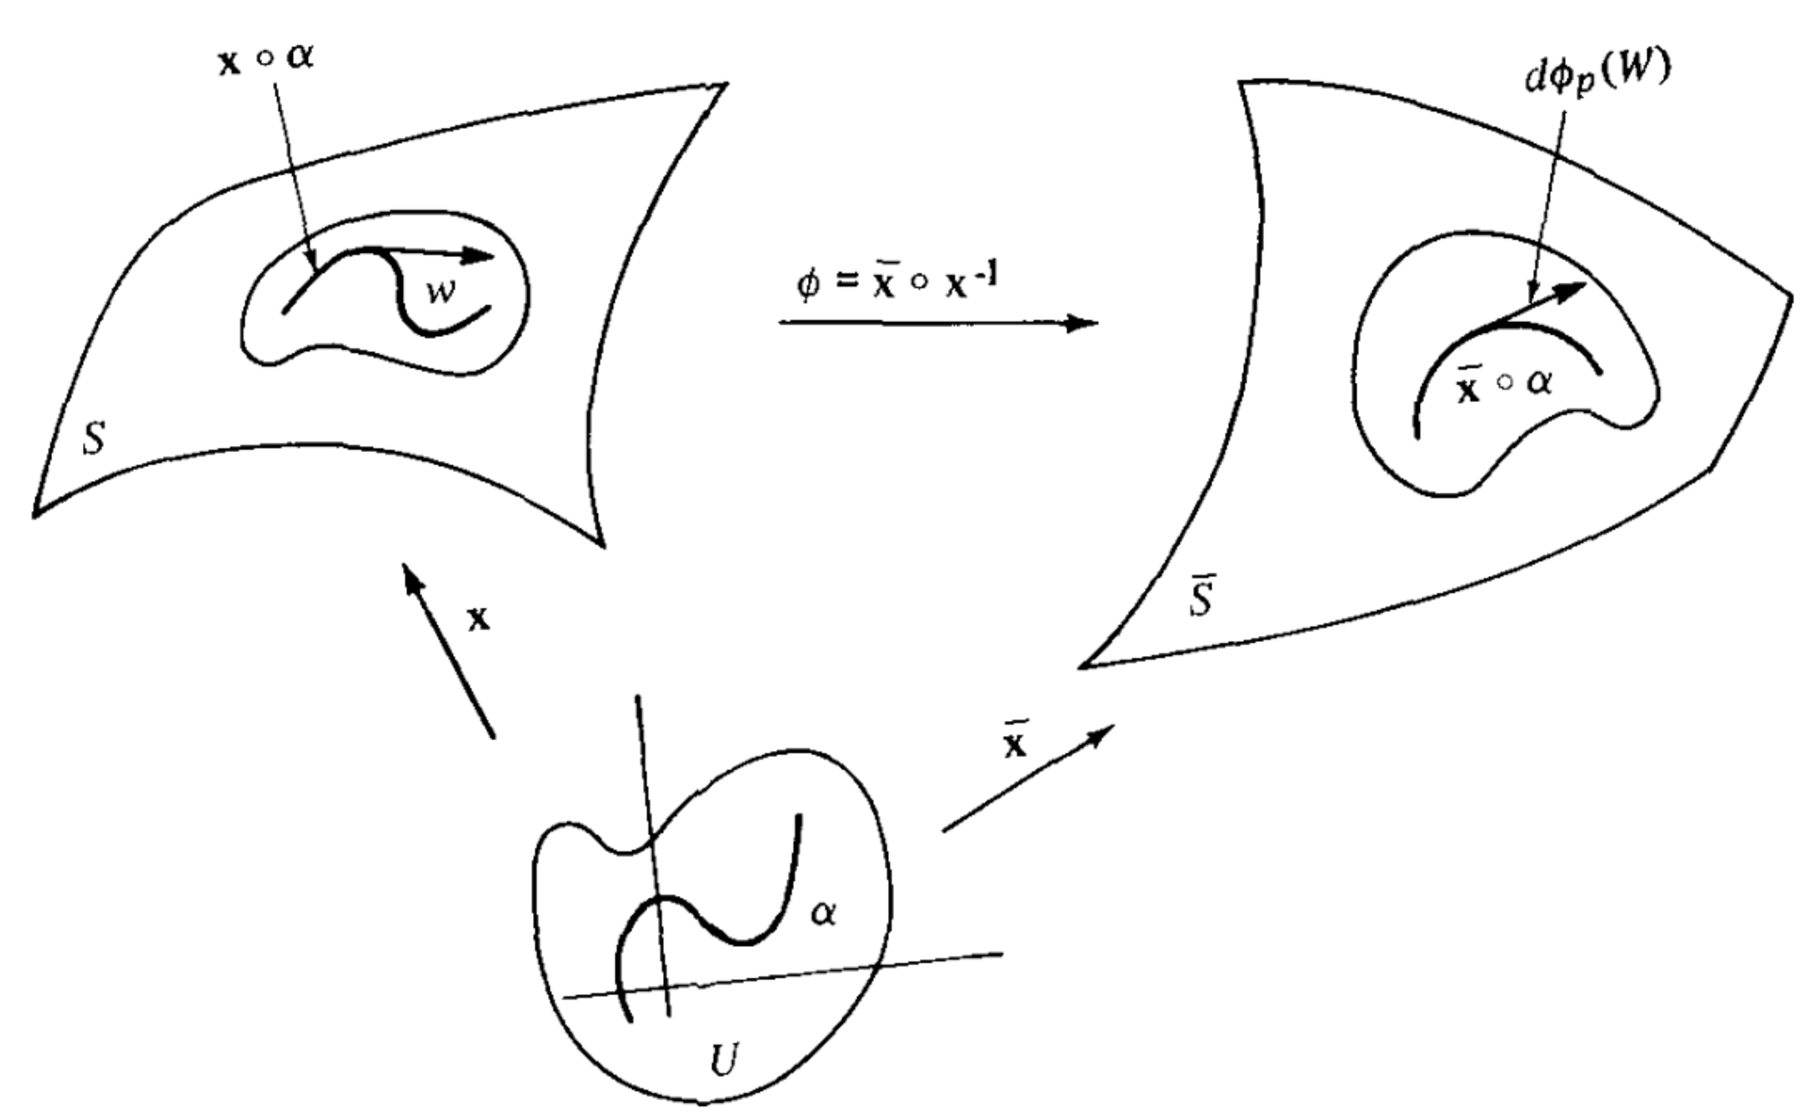
\includegraphics[scale=0.4]{3}
\caption{The vector $\varphi _p\left(w\right)$ is the tangent vector to the curve $\overline{ \mathbf{x}}  \circ {\mathbf{x}^{ - 1}} \circ \overline{\mathbf{x}} \left( {\alpha \left( t \right)} \right)$.}
\end{figure}
Thus, 
\begin{align}
d{\varphi _p}\left( w \right) = {\overline{\mathbf{x}} _u}u' + {\overline{\mathbf{x}} _v}v'.
\end{align}
Since
\begin{align}
{I_p}\left( w \right) &= E{\left( {u'} \right)^2} + 2Fu'v' + G{\left( {v'} \right)^2},\\
{I_{\varphi \left( p \right)}}\left( {d{\varphi _p}\left( w \right)} \right) &= \overline E {\left( {u'} \right)^2} + 2\overline F u'v' + \overline G {\left( {v'} \right)^2},
\end{align}
we conclude that 
\begin{align}
{I_p}\left( w \right) = {\lambda ^2}{I_{\varphi \left( p \right)}}\left( {d{\varphi _p}\left( w \right)} \right),
\end{align}
for all $p\in \mathbf{x}\left(U\right)$ and all $w\in T_p\left(S\right)$; hence, by \eqref{1.3}, $\varphi$ is a conformal mapping. \hfill $\square$\\

Local conformality is easily seen to be an equivalence relation; that is, if $S_1$ is locally conformal to $S_2$ and $S_2$ is locally conformal to $S_3$, then $S_1$ is locally conformal to $S_3$. 

The most important property of conformal maps is given by the following theorem.\\
\\
\textbf{Theorem 2.6.} \textit{Any two regular surfaces are locally conformal.}\\

The proof is based on the possibility of parametrizing a neighborhood of any point of a regular surface in such a way that the coefficients of the first fundamental form are
\begin{align}
E &= {\lambda ^2}\left( {u,v} \right) > 0,\\
F &= 0,\\
G &= {\lambda ^2}\left( {u,v} \right).
\end{align}
Such a coordinate system is called \textit{isothermal}. Once the existence of an isothermal coordinate system of a regular surface $S$ is assumed, $S$ is clearly locally conformal to a plane, and by composition locally conformal to any other surface. Finally, one proved that there exist isothermal coordinate systems on any regular surface.
\section{Selected Problems and Examples}
\textbf{Problem 3.1 (Exercise 4, \cite{2}, p.228).}  \textit{Use the stereographic projection to show that the sphere is locally conformal to a plane.}\\
\\
\textsc{Solution.} Firstly, we recall the notion of stereographic projection, see Exercise 16, \cite{2}, p.67.

One way to define a system of coordinates for the sphere $S^2$, given by
\begin{align}
\label{3.1}
{x^2} + {y^2} + {\left( {z - 1} \right)^2} = 1,
\end{align}
is to consider the so-called \textit{stereographic projection} $\pi :{S^2}\backslash \left\{ N \right\} \to {\mathbb{R}^2}$ which carries a point $p=\left(x,y,z\right)$ of the sphere $S^2$ minus the north pole $N=\left(0,0,2\right)$ onto the intersection of the $xy$ plane with the straight line which connects $N$ to $p$, Figure 2.
\begin{figure}[H]
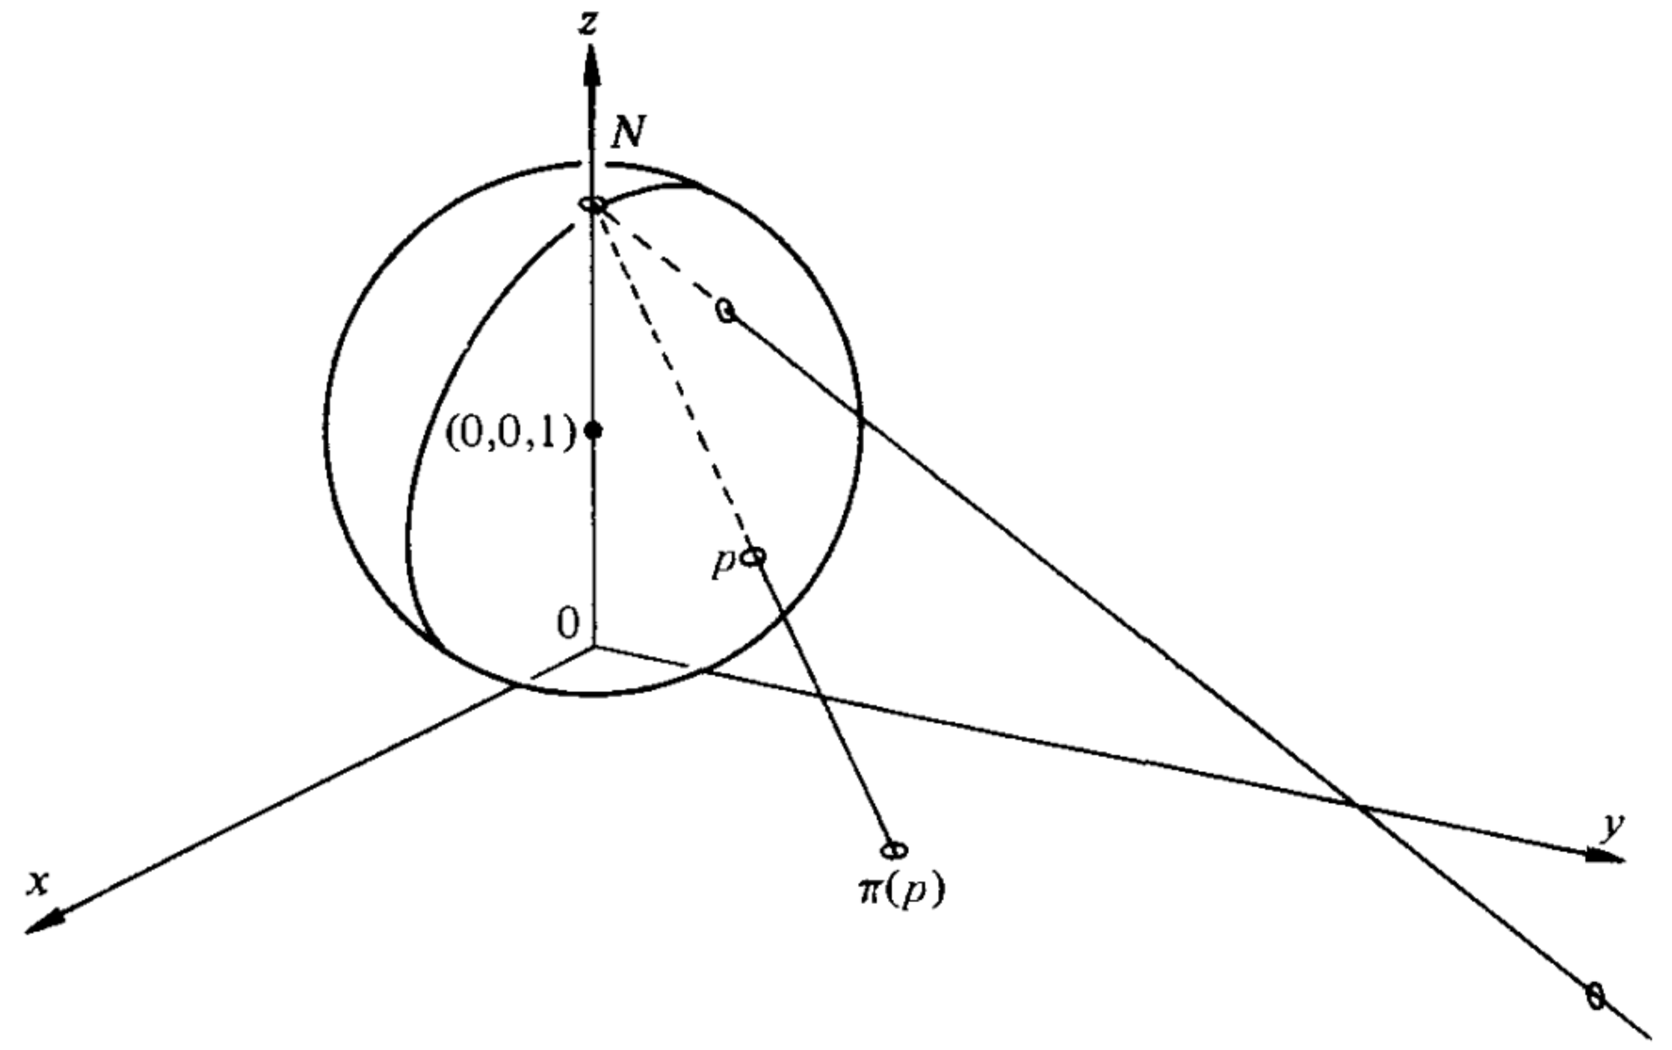
\includegraphics[scale=0.4]{4}
\caption{The stereographic projection.}
\end{figure}
Let $\left(u,v\right)=\pi \left(x,y,z\right)$, where $\left( {x,y,z} \right) \in {S^2}\backslash \left\{ N \right\}$ and $\left(u,v\right)\in xy$ plane. The inverse mapping $\pi ^{-1}$ of $\pi$ is given by
\begin{align}
x &= \frac{{4u}}{{{u^2} + {v^2} + 4}},\\
y &= \frac{{4v}}{{{u^2} + {v^2} + 4}},\\
z &= \frac{{2\left( {{u^2} + {v^2}} \right)}}{{{u^2} + {v^2} + 4}}.
\end{align}
Moreover, it is possible, using stereographic projection, to cover the sphere with two coordinate neighborhoods.

Return to our proof, we also use the sphere $S^2$ defined by \eqref{3.1} (other spheres can be handled by using an appropriate translation). Since local conformality is an equivalence relation, it suffices to prove that $\mathbb{R}^2$ is locally conformal to $S^2$. Use $\pi ^{-1}$, our parameter is given by 
\begin{align}
{\pi ^{ - 1}}:{\mathbb{R}^2} \to {S^2}\backslash \left\{ N \right\}:\mathbf{x}\left( {u,v} \right) = \left( {x\left( {u,v} \right),y\left( {u,v} \right),z\left( {u,v} \right)} \right),
\end{align}
where
\begin{align}
x\left( {u,v} \right) &= \frac{{4u}}{{{u^2} + {v^2} + 4}},\\
y\left( {u,v} \right) &= \frac{{4v}}{{{u^2} + {v^2} + 4}},\\
z\left( {u,v} \right) &= \frac{{2\left( {{u^2} + {v^2}} \right)}}{{{u^2} + {v^2} + 4}}.
\end{align}
Take $\left(u_0,v_0\right)\in \mathbb{R}^2$ and a neighborhood $V$ of $\left(u_0,v_0\right)$ arbitrarily, the mapping 
\begin{align}
\mathbf{x}:={\left. {{\pi ^{ - 1}}} \right|_V}:V &\to {S^2}\backslash \left\{ N \right\}\\
\mathbf{x}\left( {u,v} \right) &= \left( {x\left( {u,v} \right),y\left( {u,v} \right),z\left( {u,v} \right)} \right),\hspace{0.2cm}\forall \left( {u,v} \right) \in V
\end{align}
To compute the first fundamental form of $\mathbf{x}$, we need to know $\mathbf{x}_u,\mathbf{x}_v$
\begin{align}
{\mathbf{x}_u} &= \left( {\frac{{4\left( {{v^2} - {u^2} + 4} \right)}}{{{{\left( {{u^2} + {v^2} + 4} \right)}^2}}},\frac{{ - 8uv}}{{{{\left( {{u^2} + {v^2} + 4} \right)}^2}}},\frac{{16u}}{{{{\left( {{u^2} + {v^2} + 4} \right)}^2}}}} \right),\\
{\mathbf{x}_v} &= \left( {\frac{{ - 8uv}}{{{{\left( {{u^2} + {v^2} + 4} \right)}^2}}},\frac{{4\left( {{u^2} - {v^2} + 4} \right)}}{{{{\left( {{u^2} + {v^2} + 4} \right)}^2}}},\frac{{16v}}{{{{\left( {{u^2} + {v^2} + 4} \right)}^2}}}} \right).
\end{align}
From these, we obtain
\begin{align}
E &= \left\langle {{\mathbf{x}_u},{\mathbf{x}_u}} \right\rangle \\
 &= \frac{{16}}{{{{\left( {{u^2} + {v^2} + 4} \right)}^4}}}\left[ {{{\left( {{v^2} - {u^2} + 4} \right)}^2} + 4{u^2}{v^2} + 16{u^2}} \right]\\
 &= 16,\\
F &= \left\langle {{\mathbf{x}_u},{\mathbf{x}_v}} \right\rangle \\
 &= \frac{{32}}{{{{\left( {{u^2} + {v^2} + 4} \right)}^4}}}\left[ { - uv\left( {{v^2} - {u^2} + 4} \right) - uv\left( {{u^2} - {v^2} + 4} \right) + 8uv} \right]\\
 &= 0,\\
G &= \left\langle {{\mathbf{x}_v},{\mathbf{x}_v}} \right\rangle \\
 &= \frac{{16}}{{{{\left( {{u^2} + {v^2} + 4} \right)}^4}}}\left[ {4{u^2}{v^2} + {{\left( {{u^2} - {v^2} + 4} \right)}^2} + 16{v^2}} \right]\\
 &= 16,
\end{align}
i.e., $\left( {{g_{ij}}} \right) = 16\left( {\begin{array}{*{20}{c}}
1&0\\
0&1
\end{array}} \right)$, hence $\mathbf{x}$ is a conformal mapping. Since $\left(u_0,v_0\right)$ and $V$ are chosen arbitrarily, we conclude that the sphere is locally conformal to the plane. \hfill $\square$\\
\\
\textbf{Problem 3.2 (Exercise 13, \cite{2}, p.229).} \textit{Let $V$ and $W$ be finite-dimensional vectors spaces with inner products $\left\langle { \cdot , \cdot } \right\rangle $. Let $G:V\to W$ be a linear map. Prove that the following conditions are equivalent:}
\begin{enumerate}
\item \textit{There exists a real constant $\lambda \ne 0$ such that}
\begin{align}
\left\langle {G\left( {{v_1}} \right),G\left( {{v_2}} \right)} \right\rangle  = {\lambda ^2}\left\langle {{v_1},{v_2}} \right\rangle ,\hspace{0.2cm}\forall {v_1},{v_2} \in V.
\end{align}
\item \textit{There exists a real constant $\lambda >0$ such that}
\begin{align}
\left| {G\left( v \right)} \right| = \lambda \left| v \right|,\hspace{0.2cm}\forall v \in V.
\end{align}
\item \textit{There exists an orthonormal basis $\left\{ {{v_1}, \ldots ,{v_n}} \right\}$ of $V$ such that the set of vectors $\left\{ {G\left( {{v_1}} \right), \ldots ,G\left( {{v_n}} \right)} \right\}$ is an orthogonal basis of $W$ and, also, the vectors $G\left(v_i\right)$, $i=1,\ldots ,n$, have the same nonzero length.}
\end{enumerate}
\textit{If any of these conditions is satisfied, $G$ is called a \textbf{linear conformal map} (or a \textbf{similitude}).}\\
\\
\textsc{Solution.} The equivalence $\left( 1 \right) \Leftrightarrow \left( 2 \right)$ is easily deduced from the following identities
\begin{align}
\left| {G\left( v \right)} \right| &= \sqrt {\left\langle {G\left( v \right),G\left( v \right)} \right\rangle } ,\\
\left\langle {G\left( u \right),G\left( v \right)} \right\rangle  &= \frac{1}{2}\left( {{{\left| {G\left( {u + v} \right)} \right|}^2} - {{\left| {G\left( u \right)} \right|}^2} - {{\left| {G\left( v \right)} \right|}^2}} \right),
\end{align}
for all $u,v\in V$. The equivalence $\left( 1 \right) \Leftrightarrow \left( 3 \right)$ is the mollification (the additional factor $\lambda$) of the familiar result of orthogonal linear mappings in linear algebra. \hfill $\square$\\
\\
\textbf{Definition 3.3.} We say that a differentiable map $\varphi :S_1\to S_2$ \textit{preserves angles} when for every $p\in S_1$ and every pair $v_1,v_2\in T_p\left(S_1\right)$ we have
\begin{align}
\cos \left( {{v_1},{v_2}} \right) = \cos \left( {d{\varphi _p}\left( {{v_1}} \right),d{\varphi _p}\left( {{v_2}} \right)} \right).
\end{align}
\textbf{Problem 3.4 (Exercise 14, \cite{2}, p.229).} \textit{Prove that $\varphi$ is locally conformal if and only if it preserves angles.}\\
\\
\textsc{Solution.} Suppose that $\varphi$ is locally conformal, we will prove that $\varphi$ preserves angles. Indeed,
\begin{align}
\cos \left( {d{\varphi _p}\left( {{v_1}} \right),d{\varphi _p}\left( {{v_2}} \right)} \right) &= \frac{{\left\langle {d{\varphi _p}\left( {{v_1}} \right),d{\varphi _p}\left( {{v_2}} \right)} \right\rangle }}{{\left\| {d{\varphi _p}\left( {{v_1}} \right)} \right\|\left\| {d{\varphi _p}\left( {{v_2}} \right)} \right\|}}\\
  &= \frac{{{\lambda ^2}\left( p \right){{\left\langle {{v_1},{v_2}} \right\rangle }_p}}}{{\lambda \left( p \right)\left\| {{v_1}} \right\|\lambda \left( p \right)\left\| {{v_2}} \right\|}} \mbox{ by \eqref{1.5}}\\
&= \frac{{{\lambda ^2}\left( p \right){{\left\langle {{v_1},{v_2}} \right\rangle }_p}}}{{{\lambda ^2}\left( p \right)\left\| {{v_1}} \right\|\left\| {{v_2}} \right\|}}\\
& = \frac{{{{\left\langle {{v_1},{v_2}} \right\rangle }_p}}}{{\left\| {{v_1}} \right\|\left\| {{v_2}} \right\|}}\\
 &= \cos \left( {{v_1},{v_2}} \right),\hspace{0.2cm} \forall p \in {S_1},\hspace{0.2cm}\forall {v_1},{v_2} \in {T_p}\left( {{S_1}} \right).
\end{align}
i.e., $\varphi$ preserves angles.

Conversely, (see \cite{3}) suppose that $\varphi$ preserves angles, we will prove that $\varphi$ is a conformal mapping. Note that angle preserving gives
\begin{align}
\label{3.32}
\frac{{\left\langle {d{\varphi _p}\left( {{v_1}} \right),d{\varphi _p}\left( {{v_2}} \right)} \right\rangle }}{{\left\| {d{\varphi _p}\left( {{v_1}} \right)} \right\|\left\| {d{\varphi _p}\left( {{v_2}} \right)} \right\|}} = \frac{{{{\left\langle {{v_1},{v_2}} \right\rangle }_p}}}{{\left\| {{v_1}} \right\|\left\| {{v_2}} \right\|}},\hspace{0.2cm} \forall p \in {S_1},\hspace{0.2cm}\forall {v_1},{v_2} \in {T_p}\left( {{S_1}} \right).
\end{align}
Taking an orthonormal basis, $e_1,e_2$ for $T_p\left(S\right)$ and choosing a general pair of vectors
\begin{align}
{v_1} &= {e_1},\\
{v_2} &= \cos \theta {e_1} + \sin \theta {e_2},
\end{align}
which $v_2$ is a general vector on the unit circle using some $\theta$, \eqref{3.32} then implies that
\begin{align}
\frac{{\left\langle {d{\varphi _p}\left( {{e_1}} \right),d{\varphi _p}\left( {\cos \theta {e_1} + \sin \theta {e_2}} \right)} \right\rangle }}{{\left\| {d{\varphi _p}\left( {{e_1}} \right)} \right\|\left\| {d{\varphi _p}\left( {\cos \theta {e_1} + \sin \theta {e_2}} \right)} \right\|}} = \frac{{{{\left\langle {{e_1},\cos \theta {e_1} + \sin \theta {e_2}} \right\rangle }_p}}}{{\left\| {{e_1}} \right\|\left\| {\cos \theta {e_1} + \sin \theta {e_2}} \right\|}},
\end{align}
i.e., 
\begin{align}
\label{3.36}
\cos \theta  &= \frac{{\cos \theta \left\langle {d{\varphi _p}\left( {{e_1}} \right),d{\varphi _p}\left( {{e_1}} \right)} \right\rangle  + \sin \theta \left\langle {d{\varphi _p}\left( {{e_1}} \right),d{\varphi _p}\left( {{e_2}} \right)} \right\rangle }}{{\left\| {d{\varphi _p}\left( {{e_1}} \right)} \right\|\left\| {\cos \theta d{\varphi _p}\left( {{e_1}} \right) + \sin \theta d{\varphi _p}\left( {{e_2}} \right)} \right\|}}\\
 &= \frac{{\cos \theta \left\langle {d{\varphi _p}\left( {{e_1}} \right),d{\varphi _p}\left( {{e_1}} \right)} \right\rangle  + \sin \theta \left\langle {d{\varphi _p}\left( {{e_1}} \right),d{\varphi _p}\left( {{e_2}} \right)} \right\rangle }}{{\left\| {d{\varphi _p}\left( {{e_1}} \right)} \right\|{{\left( \begin{array}{l}
{\cos ^2}\theta {\left\| {d{\varphi _p}\left( {{e_1}} \right)} \right\|^2} + {\sin ^2}\theta {\left\| {d{\varphi _p}\left( {{e_2}} \right)} \right\|^2}\\
 + 2\sin \theta \cos \theta \left\langle {d{\varphi _p}\left( {{e_1}} \right),d{\varphi _p}\left( {{e_2}} \right)} \right\rangle 
\end{array} \right)}^{\frac{1}{2}}}}}. \label{3.37}
\end{align}
Setting
\begin{align}
\label{3.38}
\left\langle {d{\varphi _p}\left( {{e_1}} \right),d{\varphi _p}\left( {{e_1}} \right)} \right\rangle  &= {\lambda _1},\\
\left\langle {d{\varphi _p}\left( {{e_1}} \right),d{\varphi _p}\left( {{e_2}} \right)} \right\rangle  &= \mu ,\\
\left\langle {d{\varphi _p}\left( {{e_2}} \right),d{\varphi _p}\left( {{e_2}} \right)} \right\rangle  &= {\lambda _2}, \label{3.40}
\end{align}
then \eqref{3.36}-\eqref{3.37} becomes
\begin{align}
\label{3.41}
\cos \theta  = \frac{{{\lambda _1}\cos \theta  + \mu \sin \theta }}{{\sqrt {{\lambda _1}\left( {{\lambda _1}{{\cos }^2}\theta  + 2\mu \sin \theta \cos \theta  + {\lambda _2}{{\sin }^2}\theta } \right)} }}.
\end{align}
Taking $\theta =\frac{\pi}{2}$ with \eqref{3.41} gives
\begin{align}
0 = \frac{\mu }{{\sqrt {{\lambda _1}{\lambda _2}} }}.
\end{align}
Hence, $\mu =0$. Substituting $\mu =0$ into \eqref{3.41} yields
\begin{align}
\cos \theta  = \frac{{{\lambda _1}\cos \theta }}{{\sqrt {{\lambda _1}\left( {{\lambda _1}{{\cos }^2}\theta  + {\lambda _2}{{\sin }^2}\theta } \right)} }}.
\end{align}
Equivalently, 
\begin{align}
{\cos ^2}\theta \left( {{\lambda _1}{{\cos }^2}\theta  + {\lambda _2}{{\sin }^2}\theta  - {\lambda _1}} \right) = 0.
\end{align}
This gives
\begin{align}
\label{3.45}
{\lambda _1}{\cos ^2}\theta  + {\lambda _2}{\sin ^2}\theta  = {\lambda _1}\mbox{ for } \theta  \ne \frac{\pi }{2} + n\pi , \hspace{0.2cm} n \in \mathbb{Z}
\end{align}
Since the identity \eqref{3.45} is made of continuous functions of $\theta$ and holds for a dense set, it must also hold at the points $\theta = \frac{\pi }{2} + n\pi$ with $n \in \mathbb{Z}$. 

Finally taking $\theta =\frac{\pi}{2}$ (or taking $\theta  = \frac{\pi }{4} + n\frac{\pi }{2}$ with $n\in \mathbb{Z}$ to obtain ${\cos ^2}\theta  = {\sin ^2}\theta  = \frac{1}{2}$, or any $\theta$ such that $\sin \theta \ne 0$) in \eqref{3.45} gives $\lambda _1=\lambda _2$. We set $\lambda :=\lambda _1=\lambda_2$. And \eqref{3.38}-\eqref{3.40} then becomes
\begin{align}
\label{3.46}
\left\langle {d{\varphi _p}\left( {{e_1}} \right),d{\varphi _p}\left( {{e_1}} \right)} \right\rangle  &= \lambda ,\\
\left\langle {d{\varphi _p}\left( {{e_1}} \right),d{\varphi _p}\left( {{e_2}} \right)} \right\rangle  &= 0,\\
\left\langle {d{\varphi _p}\left( {{e_2}} \right),d{\varphi _p}\left( {{e_2}} \right)} \right\rangle  &= \lambda , \label{3.48}
\end{align}
For arbitrary $v_1,v_2\in T_p\left(S_1\right)$, we write $v_1,v_2$ in the orthonormal basis $e_1,e_2$ as
\begin{align}
{v_1} &= {v_{1,1}}{e_1} + {v_{1,2}}{e_2},\\
{v_2} &= {v_{2,1}}{e_1} + {v_{2,2}}{e_2}.
\end{align}
Then, by the linearity of the inner product $\left\langle { \cdot , \cdot } \right\rangle $, we have
\begin{align}
&\ \left\langle {d{\varphi _p}\left( {{v_1}} \right),d{\varphi _p}\left( {{v_2}} \right)} \right\rangle  \\
=&\ \left\langle {d{\varphi _p}\left( {{v_{1,1}}{e_1} + {v_{1,2}}{e_2}} \right),d{\varphi _p}\left( {{v_{2,1}}{e_1} + {v_{2,2}}{e_2}} \right)} \right\rangle \\
 =&\ \left\langle {{v_{1,1}}d{\varphi _p}\left( {{e_1}} \right) + {v_{1,2}}d{\varphi _p}\left( {{e_2}} \right),{v_{2,1}}d{\varphi _p}\left( {{e_1}} \right) + {v_{2,2}}d{\varphi _p}\left( {{e_2}} \right)} \right\rangle \\
 =&\ {v_{1,1}}{v_{2,1}}\left\langle {d{\varphi _p}\left( {{e_1}} \right),d{\varphi _p}\left( {{e_1}} \right)} \right\rangle  + {v_{1,1}}{v_{2,2}}\left\langle {d{\varphi _p}\left( {{e_1}} \right),d{\varphi _p}\left( {{e_2}} \right)} \right\rangle \\
 &+ {v_{1,2}}{v_{2,1}}\left\langle {d{\varphi _p}\left( {{e_1}} \right),d{\varphi _p}\left( {{e_2}} \right)} \right\rangle  + {v_{1,2}}{v_{2,2}}\left\langle {d{\varphi _p}\left( {{e_2}} \right),d{\varphi _p}\left( {{e_2}} \right)} \right\rangle \\
 =&\ \lambda \left( {{v_{1,1}}{v_{2,1}} + {v_{1,2}}{v_{2,2}}} \right),  \mbox{ by \eqref{3.46}-\eqref{3.48}}\\
 =&\ \lambda \left\langle {{v_1},{v_2}} \right\rangle .
\end{align}
Therefore, $\varphi$ is a conformal map. \hfill $\square$\\
\\
\textbf{Problem 3.5 (Exercise 15, \cite{2}, p.230).} \textit{Let $\varphi :\mathbb{R}^2\to \mathbb{R}^2$ be given by $\varphi \left( {x,y} \right) = \left( {u\left( {x,y} \right),v\left( {x,y} \right)} \right)$, where $u$ and $v$ are differentiable functions that satisfy the Cauchy-Riemann equations}
\begin{align}
\label{3.58}
{u_x} &= {v_y},\\
{u_y} &=  - {v_x}. \label{3.59}
\end{align}
\textit{Show that $\varphi$ is a local conformal map from $\mathbb{R}^2-Q$ into $\mathbb{R}^2$, where}
\begin{align}
Q = \left\{ {\left( {x,y} \right) \in {\mathbb{R}^2};u_x^2 + u_y^2 = 0} \right\}.
\end{align}
\textsc{Solution.} (Briefly) We compute the coefficients of the first fundamental of $\varphi$,
\begin{align}
{\varphi _x} &= \left( {{u_x},{v_x}} \right),\\
{\varphi _y} &= \left( {{u_y},{v_y}} \right),\\
E &= \left\langle {{\varphi _x},{\varphi _x}} \right\rangle  = u_x^2 + v_x^2,\\
F &= \left\langle {{\varphi _x},{\varphi _y}} \right\rangle  = {u_x}{u_y} + {v_x}{v_y},\\
G &= \left\langle {{\varphi _y},{\varphi _y}} \right\rangle  = u_y^2 + v_y^2.
\end{align}
Then the conclusion is easily deduced by combining this with the Cauchy-Riemann equations \eqref{3.58}-\eqref{3.59},
\begin{align}
G &= u_y^2 + v_y^2 = {\left( { - {v_x}} \right)^2} + u_x^2 = E,\\
F &= {u_x}{u_y} + {v_x}{v_y} =  - {u_x}{v_x} + {v_x}{u_x} = 0.
\end{align}
This completes our proof. \hfill $\square$\\
\\
\textbf{Example 3.6 (Exercise 16, \cite{2}, p.230).} Let $\mathbf{x}:U\subset \mathbb{R}^2\to \mathbb{R}^3$, where
\begin{align}
U &= \left\{ {\left( {\theta ,\varphi } \right) \in {\mathbb{R}^2};0 < \theta  < \pi ,0 < \varphi  < 2\pi } \right\},\\
\mathbf{x}\left( {\theta ,\varphi } \right)& = \left( {\sin \theta \cos \varphi ,\sin \theta \sin \varphi ,\cos \theta } \right),
\end{align}
be a parametrization of the unit sphere $S^2$. Let
\begin{align}
\log \tan \frac{1}{2}\theta  &= u,\\
\varphi  &= v,
\end{align}
and show that a new parametrization of the coordinate neighborhood $\mathbf{x}\left(U\right)=V$ can be given by
\begin{align}
\mathbf{y}\left( {u,v} \right) = \left( {{\mathop{\rm sech}\nolimits} u\cos v,{\mathop{\rm sech}\nolimits} u\sin v,\tanh u} \right).
\end{align}
It can be proved that in the parametrization $\mathbf{y}$ the coefficients of the first fundamental form are
\begin{align}
E = G = {{\mathop{\rm sech}\nolimits} ^2}u,\hspace{0.2cm} F = 0.
\end{align}
Thus, ${\mathbf{y}^{ - 1}}:V \subset {S^2} \to {\mathbb{R}^2}$ is a conformal map which takes the meridians and parallels of $S^2$ into straight lines of the plane. This is called \textit{Mercator's projection}.\\
\\
\textbf{Definition 3.7.} A diffeomorphism $\varphi :S\to \overline{S}$ is said to be \textit{area-preserving} if the area of any region $R\subset S$ is equal to the area of $\varphi \left(R\right)$.\\
\\
\textbf{Problem 3.8 (Exercise 18, \cite{2}, p.230).} \textit{Prove that if $\varphi$ is area-preserving and conformal, then $\varphi$ is an isometry.}\\
\\
\textsc{Solution.} Given two regular surfaces $S,\overline{S}$, let $U\subset \mathbb{R}^2$ be an open set, $x:U\to \mathbb{R}^3$ be a parametrization of the surface $S$ (thus $S=x\left(U\right)$), and $\varphi :S\to \overline{S}$ be an area-preserving and conformal mapping. Since $\varphi$ is a diffeomorphism between two regular surfaces $S,\overline{S}$, we can choose $\overline x  = \varphi  \circ x:U \to \overline S $ as a parametrization of $\overline{S}$ (thus $\overline{S}=\overline{x}\left(U\right)$). Take an arbitrary subset $R\subset S$ for which $R$ is also a ``region'', we denote $\left( {{g_{ij}}} \right),\left( {{{\overline g }_{ij}}} \right)$ the matrices of the first fundamental forms of $x$ and $\overline{x}$, respectively. By definition 3.1, \cite{1}, p.62, we have
\begin{align}
\label{3.74}
\mbox{Area}\left( R \right) &= \int {\int_R {dA} } \\
 &= \int {\int_{{x^{ - 1}}\left( R \right)} {\sqrt {\det \left( {{g_{ij}}} \right)} dudv} } ,\\
\mbox{Area}\left( {\varphi \left( R \right)} \right) &= \int {\int_{\varphi \left( R \right)} {d\overline A } } \\
 &= \int {\int_{{{\overline x }^{ - 1}}\left( {\varphi \left( R \right)} \right)} {\sqrt {\det \left( {{{\overline g }_{ij}}} \right)} dudv} } \\
 &= \int {\int_{{x^{ - 1}} \circ {\varphi ^{ - 1}} \circ \varphi \left( R \right)} {\sqrt {\det \left( {{{\overline g }_{ij}}} \right)} dudv} } \\
 &= \int {\int_{{x^{ - 1}}\left( R \right)} {\sqrt {\det \left( {{{\overline g }_{ij}}} \right)} dudv} } , \label{3.79}
\end{align}
where $dA, d\overline{A}$ denote the are area forms of $S$ and $\overline{S}$ (in the metrics induced by the embeddings in $\mathbb{R}^3$), respectively.\footnote{We have used that ${\overline x ^{ - 1}} = {x^{ - 1}} \circ {\varphi ^{ - 1}}$ which is deduced from the definition of $\overline{x}$: $\overline x  = \varphi  \circ x$.} Since $\varphi$ is conformal (i.e., $S$ and $\overline{S}$ are conformally equivalent), by \eqref{1.3}, there exists a \textit{positive} function $\lambda :U\to \mathbb{R}$ such that
\begin{align}
\left( {{{\overline g }_{ij}}} \right) = \lambda \left( {u,v} \right)\left( {{g_{ij}}} \right),\hspace{0.2cm}\forall \left( {u,v} \right) \in U.
\end{align}
Hence, 
\begin{align}
\label{3.81}
\det \left( {{{\overline g }_{ij}}} \right) &= {\overline g _{11}}{\overline g _{22}} - {\overline g _{12}}{\overline g _{21}}\\
& = {\lambda ^2}\left( {{g_{11}}{g_{22}} - {g_{12}}{g_{21}}} \right)\\
 &= {\lambda ^2}\det \left( {{g_{ij}}} \right). \label{3.83}
\end{align}
On the other hand, since $\varphi$ is area-preserving, we have
\begin{align}
\label{3.84}
\mbox{Area}\left( R \right) = \mbox{Area}\left( {\varphi \left( R \right)} \right),\hspace{0.2cm}\forall R \subset S,\hspace{0.2cm} R \mbox{ is a region} .
\end{align}
Combining \eqref{3.74}-\eqref{3.79} with \eqref{3.81}-\eqref{3.84}  yields for an arbitrary compact subset $R\subset S$
\begin{align}
\int {\int_{{x^{ - 1}}\left( R \right)} {\sqrt {\det \left( {{g_{ij}}} \right)} dudv} }  = \int {\int_{{x^{ - 1}}\left( R \right)} {\lambda \left( {u,v} \right)\sqrt {\det \left( {{g_{ij}}} \right)} dudv} } ,
\end{align}
Equivalently,
\begin{align}
\label{3.86}
\int {\int_{{x^{ - 1}}\left( R \right)} {\left( {1 - \lambda \left( {u,v} \right)} \right)\sqrt {\det \left( {{g_{ij}}} \right)} dudv} }  = 0,\hspace{0.2cm}\forall R \subset S,\hspace{0.2cm} R \mbox{ is a region}.
\end{align}
Since $R$ is chosen arbitrarily, it follows from \eqref{3.86} that
\begin{align}
\lambda \left( {u,v} \right) = 1,\hspace{0.2cm}\forall \left( {u,v} \right) \subset U,
\end{align}
This fact indicates that $\varphi$ is an isometry. \hfill $\square$\\
\\
\textbf{Problem 3.9 (Exercise 5, \cite{1}, p.128).} \textit{A surface of rotation can always be locally parametrized in such a way that the new parametrization is angle preserving.}\\
\textsc{Hint.} Find $\psi  = \psi \left( u \right)$  with the property that $\left(u,v\right)\to f\left(\psi \left(u\right),v\right)$ is angle preserving.\\
\\
\textbf{Example 3.10.} The \textit{Mercator projection} (see Figure 3)
\begin{figure}[H]
\label{1}
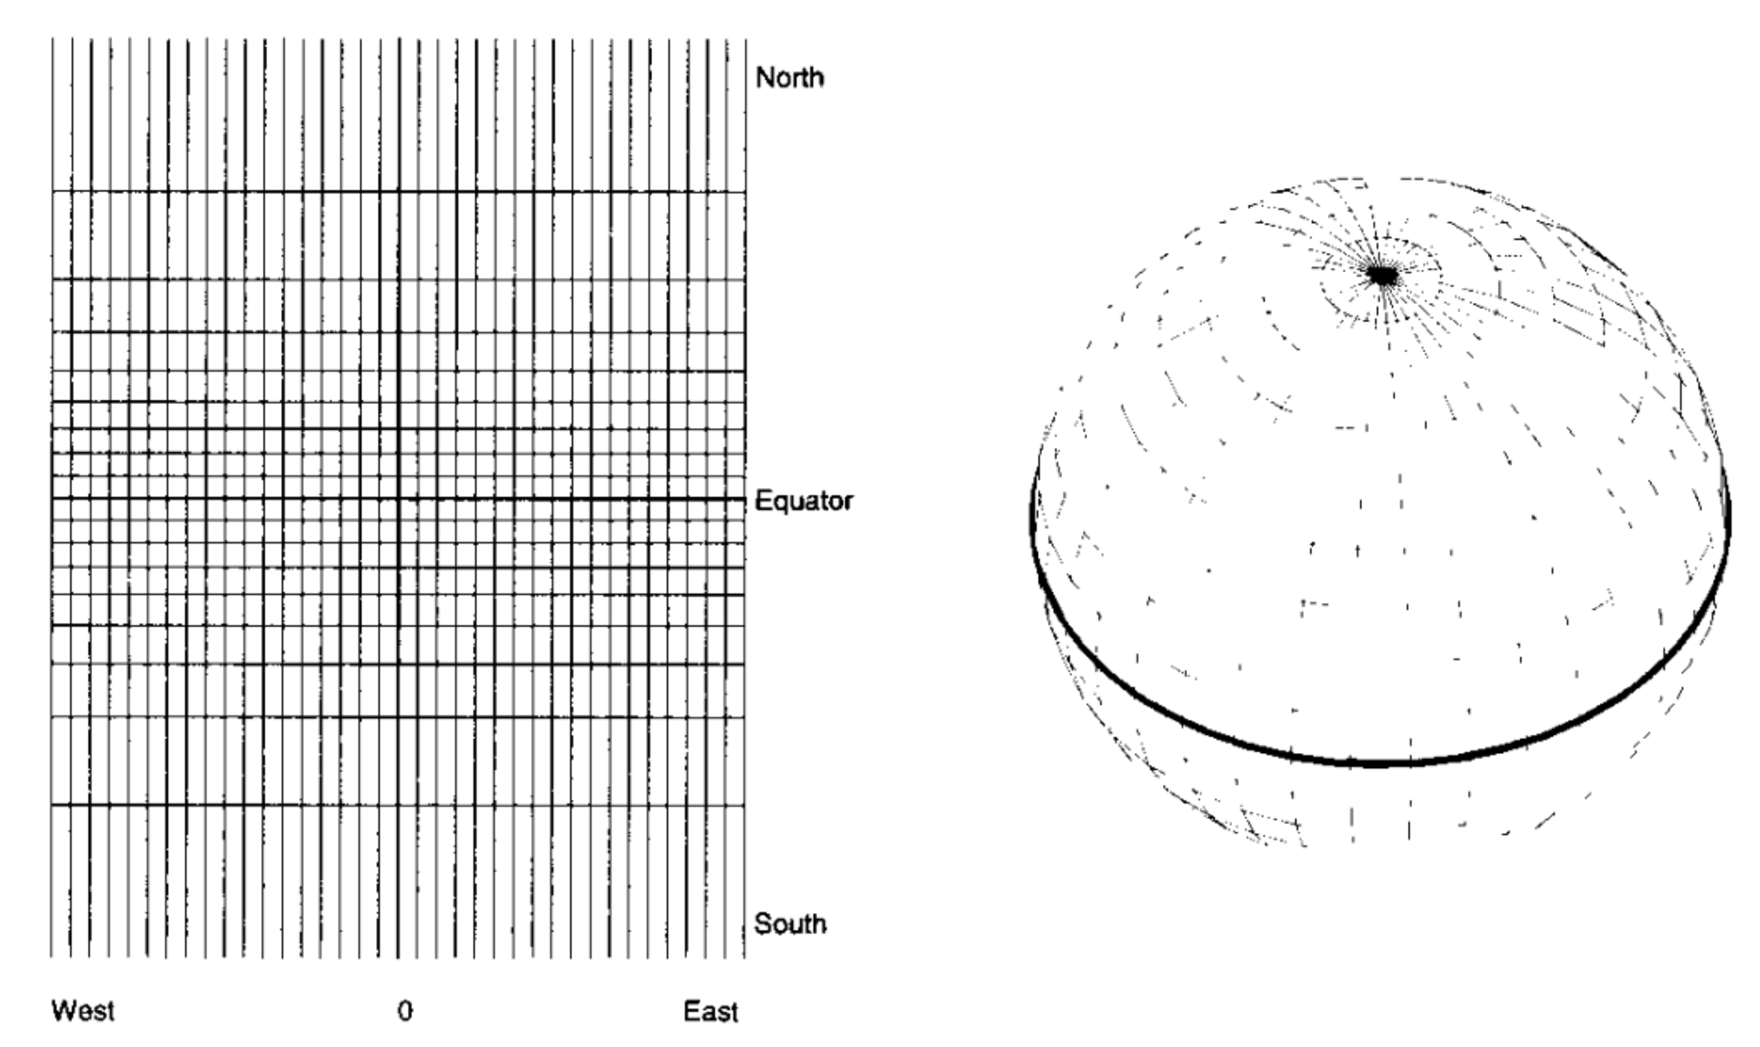
\includegraphics[scale=0.42]{1}
\caption{Coordinate grid of the Mercator projection.}
\end{figure}
\begin{align}
f\left( {u,\varphi } \right) = \frac{1}{{\cosh u}}\left( {\cos \varphi ,\sin \varphi ,\sinh u} \right)
\end{align}
is a parametrization of the surface of the sphere without the north and the south pole. It can be verified that this parametrization is angle preserving, i.e., that $u,\varphi$ are isothermal parameters. In the science of cartography, a map with this property is referred to as \textit{angle preserving} or \textit{conformal}.\\
\\
\textbf{Example 3.11 (Catenoid).} The catenoid
\begin{align}
f\left( {u,v} \right) = \left( {\cosh u\cos v,\cosh u\sin v,u} \right)
\end{align} 
is the surface of revolution generated by a catenary. Here one has
\begin{align}
{\varphi _1}\left( {u + iv} \right) &= \sinh u\cos v + i\cosh u\sin v\\
 &= \sinh \left( {u + iv} \right),\\
{\varphi _2}\left( {u + iv} \right) &= \sinh u\sin v - i\cosh u\cos v\\
 &=  - i\cosh \left( {u + iv} \right),\\
{\varphi _3}\left( {u + iv} \right) &=  - 1.
\end{align}
Clearly, $\varphi_1,\varphi_2,\varphi_3$ are holomorphic with
\begin{align}
\varphi _1^2\left( z \right) + \varphi _2^2\left( z \right) + \varphi _3^2\left( z \right) = {\sinh ^2}z + {i^2}{\cosh ^2}z + 1 = 0.
\end{align}
According to Theorem 2.2, $f$ is a conformally parametrized minimal surface. The Weierstrass representation is
\begin{align}
F\left( z \right) =  - {e^{ - z}},G =  - {e^z}.
\end{align}
\textbf{Example 3.12 (Helicoid).} The \textit{helicoid} is at the same time a ruled surface and a minimal surface
\begin{align}
h\left( {u,v} \right) = \left( {0,0, - u} \right) + v\left( { - \sin u,\cos u,0} \right) = \left( { - v\sin u,v\cos u, - u} \right).
\end{align}
Here we have standard parameters with $\lambda =1,F=0,J=0$, and this in turn implies $H=0$. However, this parametrization is not conformal. If we parametrize the surface as
\begin{align}
{h^*}\left( {u,v} \right) = \left( { - \sinh u\sin v,\sinh u\cos v, - v} \right),
\end{align}
then the complexification which this induces is
\begin{align}
{\varphi _1}\left( z \right) = i\sinh z,{\varphi _2}\left( z \right) = \cosh z,{\varphi _3}\left( z \right) = i.
\end{align}
These are exactly the same functions $\varphi_1,\varphi_2,\varphi_3$ as occurred above in the case of the catenoid, up to a factor of $i$. In particular, $h^*$ is a conformally parametrized minimal surface. We also see that the catenoid $f$ and the helicoid $h^*$ are isometric, since $g_{12}=0$ and ${g_{11}} = {g_{22}} = \frac{1}{2}\left( {{\varphi _1}\overline {{\varphi _1}}  + {\varphi _2}\overline {{\varphi _2}}  + {\varphi _3}\overline {{\varphi _3}} } \right)$, an expression which is invariant under multiplication by $i$. For this reason one speaks of \textit{conjugate pairs} of minimal surfaces, if the complexification of one is obtained by multiplication by $i$ of the other. In this sense, the catenoid and the helicoid are conjugate to one another, see Figure 4.
\begin{figure}[H]
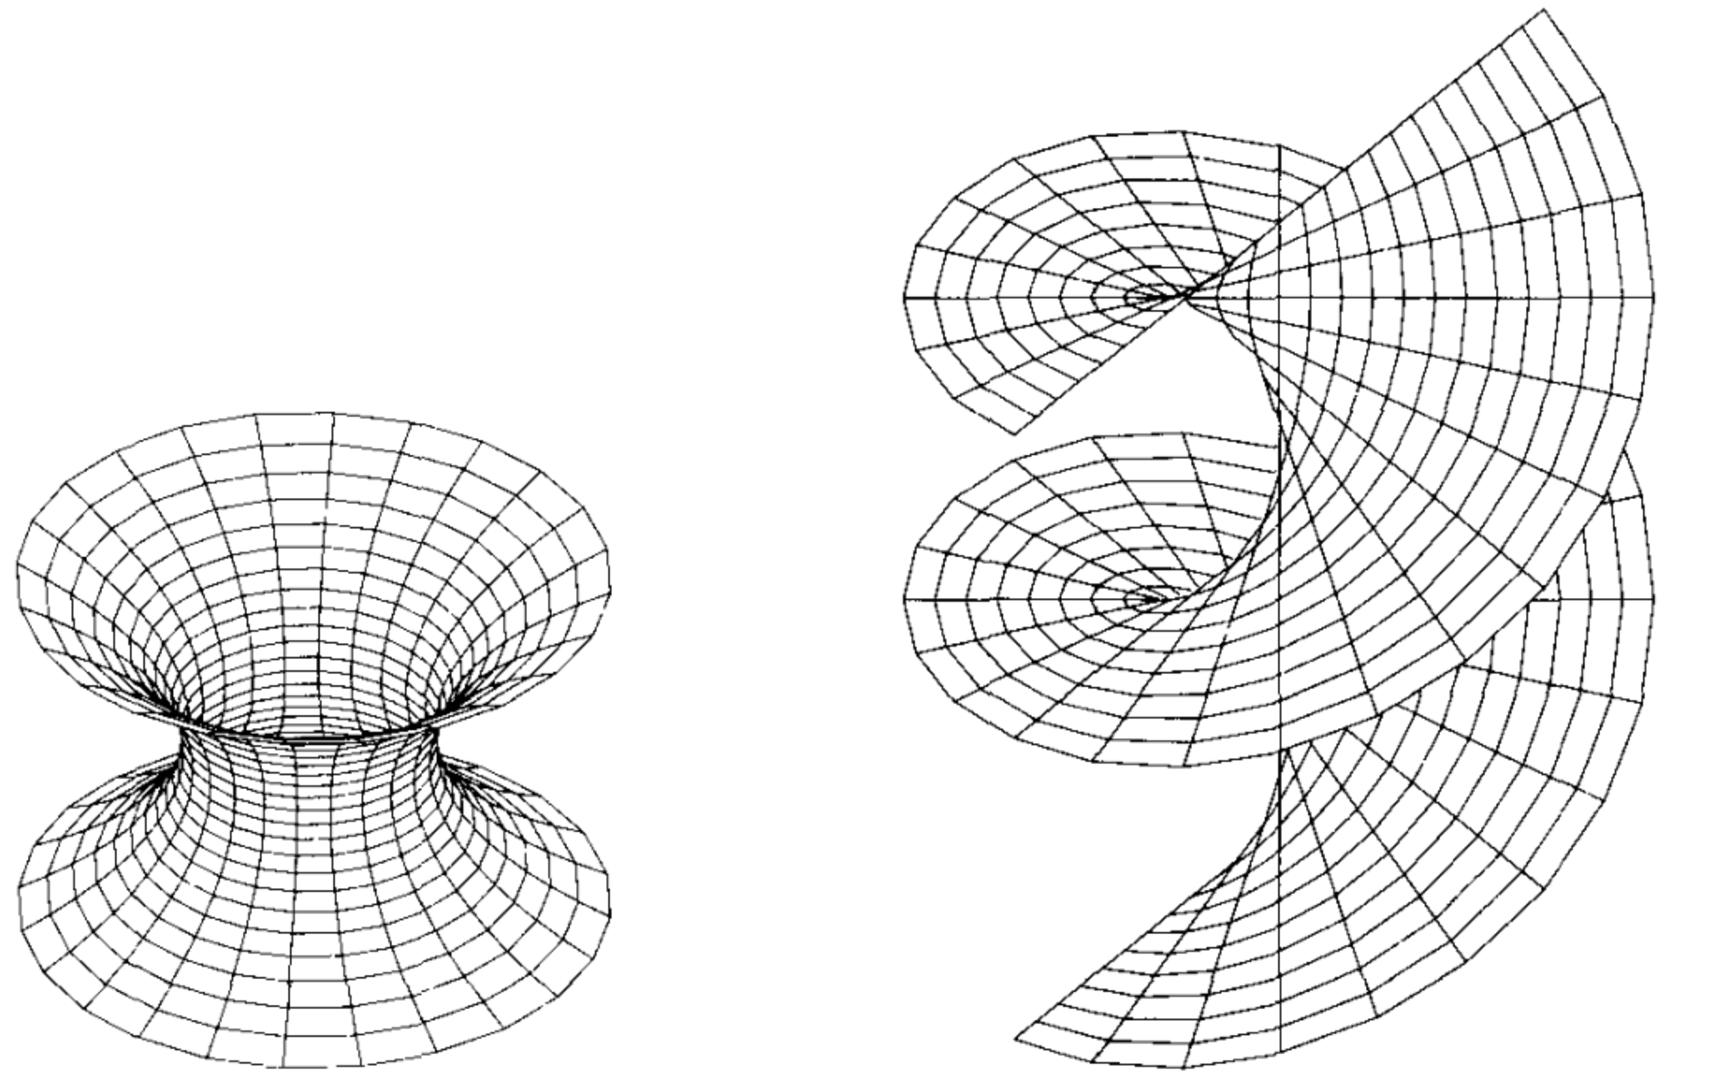
\includegraphics[scale=0.42]{2}
\caption{The interior part of a catenoid and a right helicoid (staircase surface).}
\end{figure}
One can even view both of them as the real and imaginary parts, respectively, of a common complex surface.\\
\\
\\
\\
\begin{center}
\textsc{The End}
\end{center}
\newpage
\begin{thebibliography}{999}
\bibitem {1} Wolfgang K\"{u}hnel, Differential Geometry, Curves Surfaces Manifolds, Second Edition, Student Mathematical Library, Volume 16, AMS.
\bibitem {2} Manfredo P. do Carmo, Differential Geometry of Curves and Surfaces, 1st edition, Prentice-Hall, Inc., Englewood Cliffs, New Jersey. 1976.
\bibitem {3} \url{https://math.stackexchange.com/questions/150448/proof-that-angle-preserving-map-is-conformal}
\end{thebibliography}
\end{document}